\chapter{VISUALISASI KINERJA SISWA DARI MEDIA PEMBELAJARAN DIGITAL MENGGUNAKAN PETA ORGANISASI DIRI (SOM)}

\section{Pendahuluan}

    Pendidikan adalah proses pembelajaran pengetahuan, keterampilan, atau pengalaman baru. Dalam pendidikan, siswa belajar cara memecahkan masalah. Di sini, penting bagi siswa untuk mengembangkan kemampuan kognitif dalam memahami makna masalah dan kemampuan relevan untuk memecahkannya. Kemampuan memecahkan masalah terdiri dari mengorganisir informasi yang ada dan merancang strategi untuk mengatasi masalah. Oleh karena itu, dalam memecahkan masalah, setiap siswa perlu mengembangkan proses berpikir yang unik \citep{Pamitah2015}. Di sisi lain, di sebagian besar negara, pendidikan wajib sering dilaksanakan dalam kelas besar, di mana guru kesulitan untuk memperhatikan karakteristik belajar setiap siswa.
    
    Oleh karena itu, dalam studi ini, kami berusaha mengembangkan alat pendidikan yang memungkinkan guru untuk menganalisis perilaku belajar siswa secara intuitif dan membantu guru menghasilkan saran yang berarti, terutama untuk siswa dengan prestasi rendah. Hal ini dimungkinkan oleh ketersediaan data belajar siswa yang diperoleh melalui platform belajar digital. Dalam studi ini, kami menggunakan data dari \textit{MONSAKUN} \citep{Supianto2016}, platform belajar yang digunakan di Jepang untuk mengajarkan aritmatika kepada siswa sekolah dasar. Dalam platform pembelajaran ini, setiap siswa mendapatkan kumpulan soal yang sama, namun mereka dapat mengembangkan \textit{strategi} sendiri untuk menyelesaikan soal-soal tersebut. Perbedaan strategi yang digunakan siswa dalam menyelesaikan soal-soal tersebut berasal dari cara dan proses berpikir yang berbeda-beda. Strategi pemecahan masalah mereka kemudian direkam sebagai data \textit{karakteristik pembelajaran}, di mana setiap siswa diwakili sebagai titik dalam ruang dimensi tinggi, di mana dimensi tersebut menunjukkan jumlah \textit{fitur pembelajaran}. Dalam studi kami, kami pertama-tama mengelompokkan siswa sehingga siswa dengan karakteristik pembelajaran serupa membentuk \textit{kluster}, sementara siswa yang berbeda dikelompokkan dalam kluster yang berbeda. Karena tujuan kami adalah mengembangkan alat analitis intuitif, kami perlu menyajikan kluster-kluster ini secara intuitif kepada guru yang tidak \textit{necessarily} ahli dalam analisis data, dan oleh karena itu kami mengadopsi teknik \textit{visualisasi} melalui \textit{pengurangan dimensi} (DR) \citep{Kreuseler2002a}.
    
    Ada banyak algoritma untuk teknik pengurangan dimensi (DR), di mana salah satu algoritma DR tertua adalah Analisis Komponen Utama (\textit{PCA}). PCA adalah algoritma yang mengurangi dimensi data dengan mengidentifikasi yang disebut \textit{Komponen Utama} \citep{Ringner2008}. Meskipun PCA dapat diimplementasikan dengan mudah, algoritma ini dibatasi oleh linearitas dalam menentukan Komponen Utama, sehingga mungkin tidak dapat cukup menggambarkan non-linearitas dalam data. Algoritma pengurangan dimensi konvensional lainnya adalah Analisis Diskriminan Linier (\textit{LDA}). Mirip dengan PCA, LDA juga merupakan metode DR yang dibatasi oleh linearitas, tetapi mempertimbangkan label kelas data \citep{Hartono2017}. Dalam studi ini, kami menggunakan \textit{Self-Organizing Map (SOM)} karena kemudahan implementasinya dan tidak dibatasi oleh linearitas. Selama beberapa dekade terakhir, berbagai varian \textit{SOM} telah digunakan secara luas untuk analisis dan visualisasi data, misalnya \citep{Lestari2014}. Di sini, SOM menghasilkan \textit{peta dua dimensi} yang mempertahankan urutan topologis karakteristik pembelajaran data berdimensi tinggi, di mana siswa dengan karakteristik pembelajaran yang sama ditempatkan dekat satu sama lain, sementara siswa dengan karakteristik yang sangat berbeda ditempatkan jauh satu sama lain. Hal ini terutama menarik dalam mengidentifikasi siswa berprestasi rendah, karena mereka adalah yang paling penting bagi guru untuk diberi bimbingan. Dengan menempatkan siswa berprestasi rendah dan siswa lain di sekitar mereka pada peta, guru dapat menggunakan siswa lain sebagai referensi untuk meningkatkan kinerja siswa berprestasi rendah. Ide dasarnya adalah meniru karakteristik pembelajaran siswa lain yang digunakan sebagai referensi. Karena kesamaan karakteristik pembelajaran, siswa berprestasi rendah tidak perlu melakukan perubahan drastis pada gaya belajar mereka. Diharapkan dengan mengulangi proses ini pada tugas-tugas lain, kinerja siswa akan meningkat secara bertahap.
    
    Keunggulan utama teknik \textit{visualisasi} adalah mengubah data menjadi representasi grafisnya sambil mempertahankan karakteristik aslinya untuk membantu manusia dalam melakukan penalaran visual dan pengenalan pola \citep{Bara2018}. Dalam salah satu contoh teknik \textit{visualisasi}, Supianto dkk. \citep{SupiantoHayashiHirashima2016} mendeteksi situasi penting di mana siswa mengalami hambatan belajar dan kesulitan memahami struktur masalah. Studi ini mengusulkan metode untuk memvisualisasikan tindakan siswa dari data log \textit{MONSAKUN}. Mereka menyajikan \textit{visualisasi} aktivitas siswa dalam lingkungan \textit{pembelajaran berbasis pemecahan masalah}, di mana siswa mengajukan masalah berdasarkan tugas mereka dalam bentuk grafik yang menggambarkan jumlah langkah yang diperlukan untuk mencapai jawaban yang benar. Meskipun studi ini memiliki kesamaan dengan studi sebelumnya, tujuan kami adalah mengidentifikasi siswa dengan kinerja rendah dan menghasilkan saran pembelajaran yang realistis bagi mereka.
    
    Struktur sisa makalah ini sebagai berikut: Bagian 2 menjelaskan gambaran umum SOM dan karya terkait SOM. Beberapa eksperimen \textit{visualisasi} dengan data \textit{MONSAKUN} dijelaskan di Bagian 3, sementara bagian akhir berisi kesimpulan.

\section{Gambaran Umum Peta Organisasi Diri (SOM)}

    SOM adalah jenis Jaringan Saraf Tiruan (JST) yang diperkenalkan oleh Kohonen \citep{Kohonen1998} pada tahun 1980-an. SOM telah berhasil diterapkan dalam berbagai bidang seperti kuantisasi vektor, pengenalan pola, analisis data keuangan, analisis teks lengkap dan gambar, regresi, dan diagnosis kesalahan \citep{Jin2004}.

    SOM dapat diterapkan sebagai alat \textit{visualisasi} \citep{Dragomir2014} karena mengubah hubungan statistik non-linier antara data berdimensi tinggi menjadi hubungan geometris sederhana dari titik-titik gambarnya pada tampilan berdimensi rendah.

    \begin{figure}[H]
        \centering
        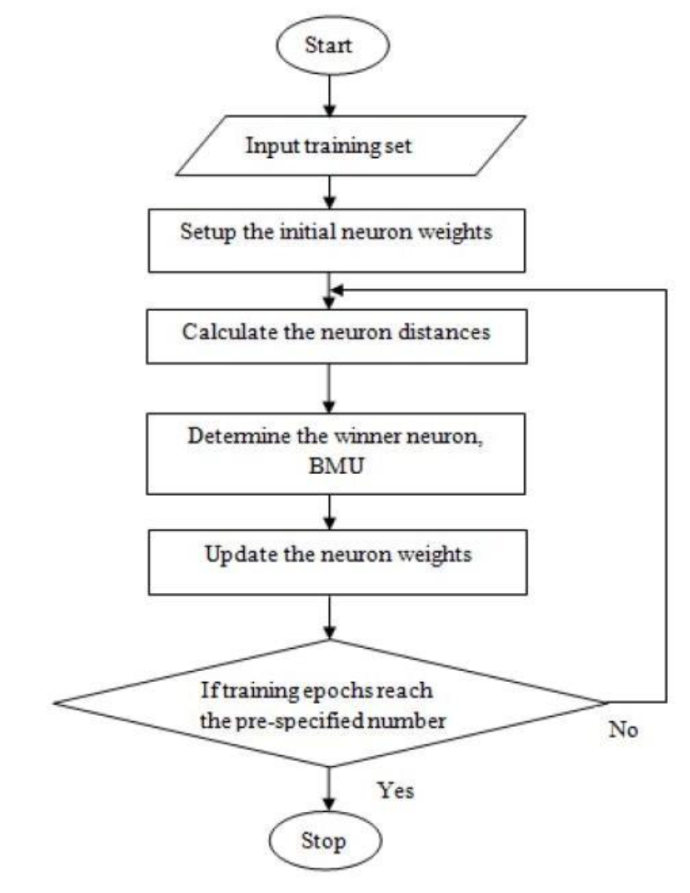
\includegraphics[width=0.7\textwidth]{Gambar/gambar5.1.png}
        \caption{Algoritma Pembelajaran SOM}
    \end{figure}

    SOM terdiri dari sekumpulan neuron buatan, masing-masing terkait dengan vektor kamus kode dengan dimensi yang sama dengan input, yang mewakili struktur topologi data berdimensi tinggi \citep{Cabanes2012}. Gambar 1 menampilkan ringkasan algoritma pembelajaran SOM \citep{Fuertes2010}. Gambar ini menunjukkan bahwa setiap instance data masukan akan diproses berdasarkan jumlah epoch pelatihan yang telah ditentukan sebelumnya. Selama pelatihan SOM, jarak antara data masukan dan vektor buku kode dihitung untuk menentukan neuron pemenang, yang disebut unit pencocokan terbaik (BMU).

    Sifat matematis perilaku pembelajaran SOM telah dijelaskan secara rinci dalam \citep{Cabanes2012} tetapi akan diuraikan secara singkat sebagai berikut :

    Misalkan $X(t) = x(x_1, x_2, \ldots, x_n)$ adalah vektor masukan berdimensi $n$, dan
    $w_i(t) = (w_{i1}, w_{i2}, \ldots, w_{im})$ adalah vektor referensi yang terkait dengan neuron ke-$i$ pada waktu $t$.

    \[
        w_{\text{in}} = \min_i \| x(t) - w_i(t) \|
    \]

    Dalam Persamaan (1), $w_{\text{in}}$ adalah indeks Unit Pencocokan Terbaik (BMU).
    
    Setelah menentukan BMU, setiap vektor referensi dimodifikasi sebagai berikut.

    \[
        w_i(t + 1) = w_i(t) + \alpha(t) \, h(w_{\text{in}}, i, t) \, [x(t) - w_i(t)]
    \]

    Dalam Persamaan~(2), $\alpha(t)$ merujuk pada laju pembelajaran yang nilainya menurun seiring dengan waktu iterasi, sedangkan $h(w_{\text{in}}, i, t)$ merujuk pada fungsi tetangga yang merupakan fungsi monoton menurun terhadap jarak geometris antara \textit{Best Matching Unit} (BMU) dan neuron ke-$j$ pada peta. 

    Fungsi tetangga ini memastikan pelestarian struktur topologis dari data masukan berdimensi tinggi ke dalam peta berdimensi rendah.
    
\section{Eksperimen Visualisasi}

    Untuk eksperimen dalam makalah ini, data yang digunakan terdiri dari karakteristik pembelajaran 39 siswa pada 5 tingkat masalah, di mana tingkat 1 terdiri dari 12 soal, tingkat 2 terdiri dari 3 soal, tingkat 3 terdiri dari 12 soal, tingkat 4 terdiri dari 3 soal, dan tingkat 5 terdiri dari 12 soal. Level 2 dan 4 tidak digunakan karena hanya terdiri dari 3 soal \citep{Hirashima2007}.

    \textit{MONSAKUN} sendiri dirancang sebagai media pembelajaran interaktif untuk pemecahan masalah \citep{Hirashima2014}. \textit{MONSAKUN} mencatat aktivitas siswa selama kegiatan pemecahan masalah mereka, yang mencakup fitur-fitur berikut:

    \begin{enumerate}
        \item Nomor Induk Mahasiswa: Ini berisi variabel kunci utama yang membedakan setiap mahasiswa.
        \item Durasi: Mengandung waktu yang dibutuhkan siswa untuk menyelesaikan tugas dalam detik.
        \item Langkah: Mengandung jumlah langkah (set dan remove) yang dilakukan oleh siswa.
        \item Set: Ini berisi jumlah langkah set yang dilakukan oleh siswa.
        \item Menghapus: Mengandung jumlah langkah menghapus yang dilakukan oleh siswa.
        \item C1: Mengandung jumlah penggunaan kartu 1 oleh siswa.
        \item C2: Menampilkan jumlah penggunaan kartu 2 oleh siswa.
        \item C3: Mengandung jumlah penggunaan kartu 3 oleh siswa
        \item C4: Menampilkan jumlah penggunaan kartu 4 oleh siswa
        \item C5: Mengandung jumlah penggunaan kartu 5 oleh siswa
        \item C6: Mengandung jumlah penggunaan kartu 6 oleh siswa
        \item Unique: Mengandung jumlah kombinasi kartu unik yang digunakan oleh siswa
        \item Error: Mengandung jumlah kesalahan selama pelaksanaan tugas
    \end{enumerate}

    Kami melatih SOM untuk setiap level pada setiap tugas untuk memvisualisasikan karakteristik siswa. Gambar 2 memvisualisasikan distribusi karakteristik siswa untuk tugas 1 (level 1). Setiap angka pada peta mewakili ID siswa tertentu. Misalnya, kita dapat secara intuitif memahami bahwa siswa 2 memiliki kesamaan perilaku belajar dengan siswa 16 tetapi sangat berbeda dari siswa 22. Di sudut kiri bawah peta, kita dapat mengamati sekelompok siswa dengan kesamaan perilaku belajar yang serupa, sementara di sisi kanan peta, kita dapat mengamati tiga siswa (31, 14, 22) yang secara jelas berbeda dari siswa lain. Siswa 7 (lingkaran biru) adalah siswa dengan kinerja terburuk. Dapat diamati bahwa siswa tersebut memiliki kesamaan dengan banyak siswa lain (6, 20, 33) dan berpotensi dapat memperoleh manfaat dengan meniru perilaku belajar mereka.

    \begin{figure}[H]
        \centering
        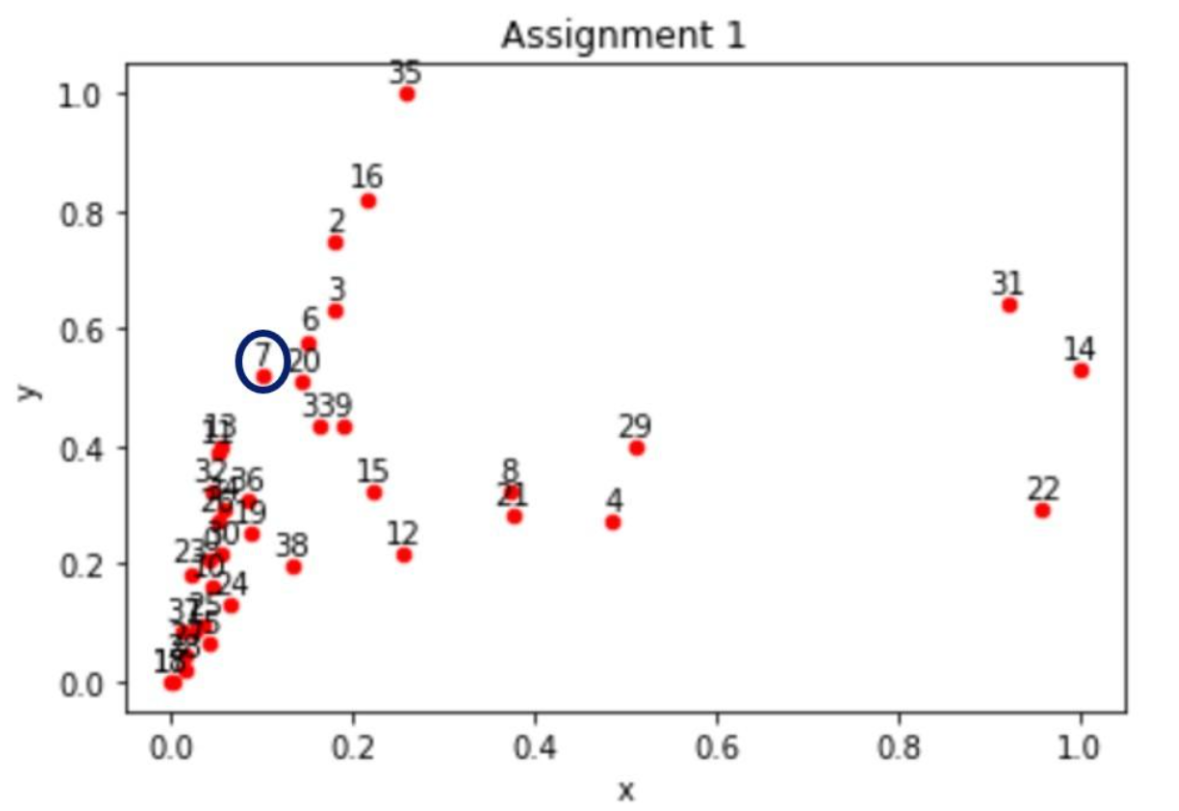
\includegraphics[width=0.7\textwidth]{Gambar/gambar5.2.png}
        \caption{Visualisasi SOM Siswa pada Tugas 1 Level 1}
    \end{figure}

    Gambar 3 menampilkan distribusi karakteristik siswa untuk tugas 4 (tingkat 1). Setiap angka pada peta mewakili ID siswa tertentu. Di sini, misalnya, kita dapat secara intuitif memahami bahwa siswa 32 memiliki kesamaan perilaku belajar dengan siswa 7 tetapi sangat berbeda dari siswa 28. Di sudut kiri bawah peta, kita dapat mengamati sekelompok siswa dengan kesamaan perilaku belajar yang serupa, sementara di sisi kanan peta, kita dapat mengamati satu siswa (28) yang secara jelas berbeda dari siswa lainnya. Siswa 13 (lingkaran biru) adalah siswa dengan kinerja terburuk

    Dapat diamati bahwa siswa tersebut memiliki kesamaan dengan banyak siswa lain (24, 10, 30) dan berpotensi mendapatkan manfaat dengan meniru perilaku belajar mereka.

    \begin{figure}[H]
        \centering
        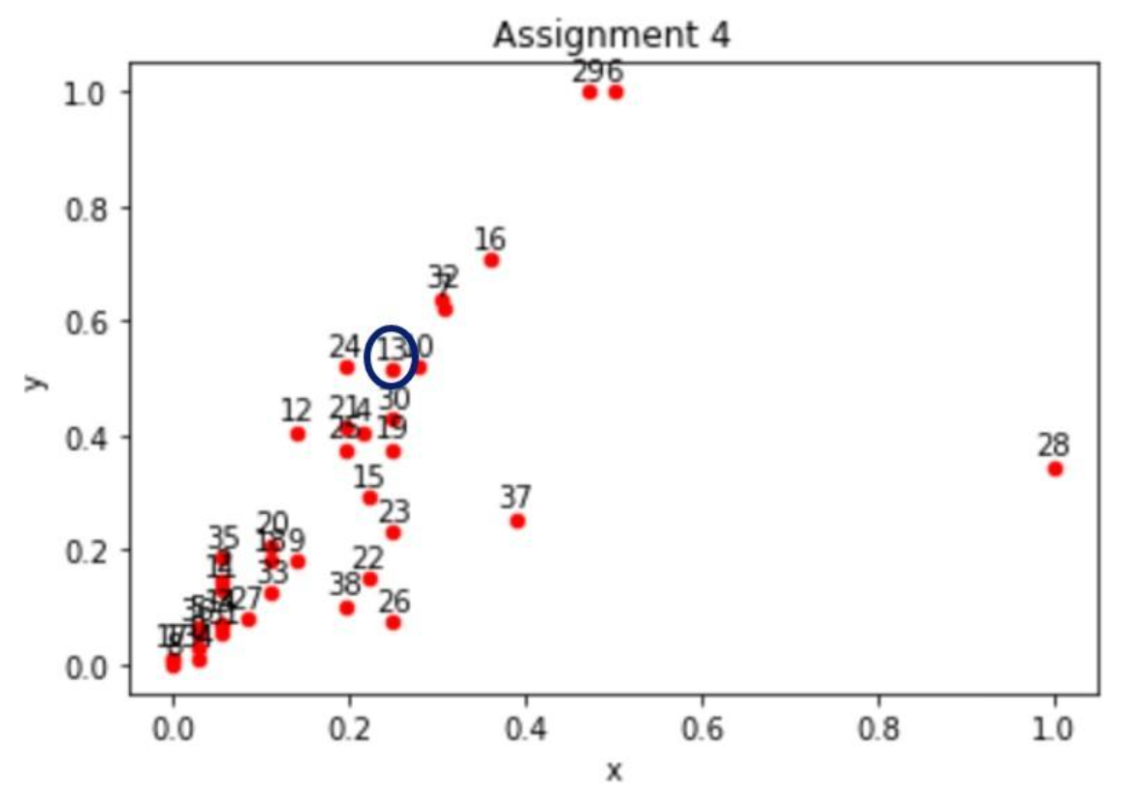
\includegraphics[width=0.7\textwidth]{Gambar/gambar5.3.png}
        \caption{Visualisasi SOM Siswa pada Tugas 4 Level 1}
    \end{figure}

\section{Kesimpulan}

    Dalam makalah ini, kami telah melakukan eksperimen awal dalam memvisualisasikan karakteristik siswa. Meskipun peta yang dihasilkan intuitif dan dalam beberapa hal informatif untuk memahami karakteristik siswa, peta tersebut hanya memberikan gambaran sekilas untuk satu tes tertentu. Dalam penelitian kami selanjutnya, kami berencana mengintegrasikan informasi dari peta ini ke dalam grafik kesamaan yang lebih baik menggambarkan kesamaan siswa secara hierarkis. Kami kemudian akan menggunakan grafik-grafik ini untuk secara otomatis menghasilkan saran pembelajaran yang dapat disesuaikan secara manual oleh guru dengan tujuan utama membantu siswa.
    
    Kami juga berencana untuk membangun antarmuka yang intuitif dan interaktif yang memungkinkan guru untuk dengan mudah menggunakan alat saran ini. Sistem penasihat akan diimplementasikan dan dievaluasi secara menyeluruh di Indonesia
